% ══════════════════════════════════════════════════════════════════
\chapter{The Gradient Trap: Forward-Backward Asymmetry}
\label{ch:gradient_trap}
% ══════════════════════════════════════════════════════════════════

\noindent
\textbf{Experimental setup.}
50 hidden layers, width~784, Fashion-MNIST (2000~samples).
We compare three initializers: He (baseline),
\texttt{row\_centered\_he\_var\_adj}, and
\texttt{row\_centered\_forward\_balanced}.

% ──────────────────────────────────────────────────────────────────
\section{The Centering Ratio: $(\pi-1)/\pi$}
\label{sec:centering_ratio}

\subsection{Half-Gaussian moments}

After ReLU, the activations follow a half-Gaussian distribution.
If the pre-activation $z \sim \mathcal{N}(0, \sigma^2)$, then
$a = \relu(z) = \max(0,z)$ satisfies:

\begin{lemma}[Half-Gaussian moments]
\label{lem:half_gaussian}
\begin{equation}\label{eq:half_gauss_moments}
  \E[a] = \frac{\sigma}{\sqrt{2\pi}},
  \qquad
  \E[a^2] = \frac{\sigma^2}{2}.
\end{equation}
\end{lemma}

\begin{proof}
Since $\Pr(z > 0) = 1/2$ and the positive half of $\mathcal{N}(0,\sigma^2)$
is a half-normal distribution:
\[
  \E[a] = \E[z \mid z > 0] \cdot \Pr(z > 0)
  = \frac{\sigma\sqrt{2/\pi}}{1} \cdot \frac{1}{2}
  = \frac{\sigma}{\sqrt{2\pi}}.
\]
For the second moment:
$\E[a^2] = \E[z^2 \mid z > 0]\cdot\Pr(z > 0) = \sigma^2 \cdot \frac{1}{2}$.
\end{proof}

From these moments, the variance of a post-ReLU activation is:
\begin{equation}\label{eq:var_a}
  \Var(a) = \E[a^2] - (\E[a])^2
  = \frac{\sigma^2}{2} - \frac{\sigma^2}{2\pi}
  = \frac{\sigma^2}{2}\left(1 - \frac{1}{\pi}\right)
  = \frac{\sigma^2(\pi - 1)}{2\pi}.
\end{equation}

\subsection{Why the centering ratio matters}

Before stating the centering ratio formally, let us explain
\emph{why} this quantity is the key to understanding the gradient trap.

Post-ReLU activations are always non-negative ($a_j \geq 0$), so
they have a positive mean $\E[a] > 0$.
This mean is a \emph{constant offset} --- it depends on the weight
variance $\sigma^2$ but not on which input $\bm{x}$ was fed in.
It carries no information about the class of the input.

Recall from equation~\eqref{eq:rc_motivation} that row-centered
weights ($\sum_j W_{ij} = 0$) are blind to any constant component
in their input.  So row-centered weights can only access the
\emph{varying} part of the activations --- the variance $\Var(a)$.

The centering ratio $\Var(a)/\E[a^2]$ answers a precise question:
\emph{what fraction of the total activation energy is accessible to
row-centered weights?}

\emph{Why $\E[a^2]$ and not $\E[a]$?}  Signal propagation depends
on \emph{energy} (second moments), not first moments.  The forward
gain (Definition~\ref{def:activation_matrix}) compares
$\E[(a^{(l)})^2]$ across layers, so the relevant question is what
fraction of \emph{energy} is available, not what fraction of the
\emph{mean} is available.

\begin{proposition}[Centering ratio]
\label{prop:centering_ratio}
For post-ReLU activations with pre-activation $z \sim \mathcal{N}(0,\sigma^2)$:
\begin{equation}\label{eq:centering_ratio}
  \frac{\Var(a)}{\E[a^2]}
  = \frac{\sigma^2(\pi-1)/(2\pi)}{\sigma^2/2}
  = \frac{\pi - 1}{\pi}
  \approx 0.6817.
\end{equation}
This ratio is \textbf{independent of $\sigma$} --- it is a universal
property of the ReLU activation function.
\end{proposition}

\noindent
\textbf{Interpretation.}
Out of the total signal energy $\E[a^2]$, only $68.2\%$ is accessible
to row-centered weights.  The remaining $31.8\%$ is the constant DC
offset that gets ignored.

\begin{figure}[h]
\centering
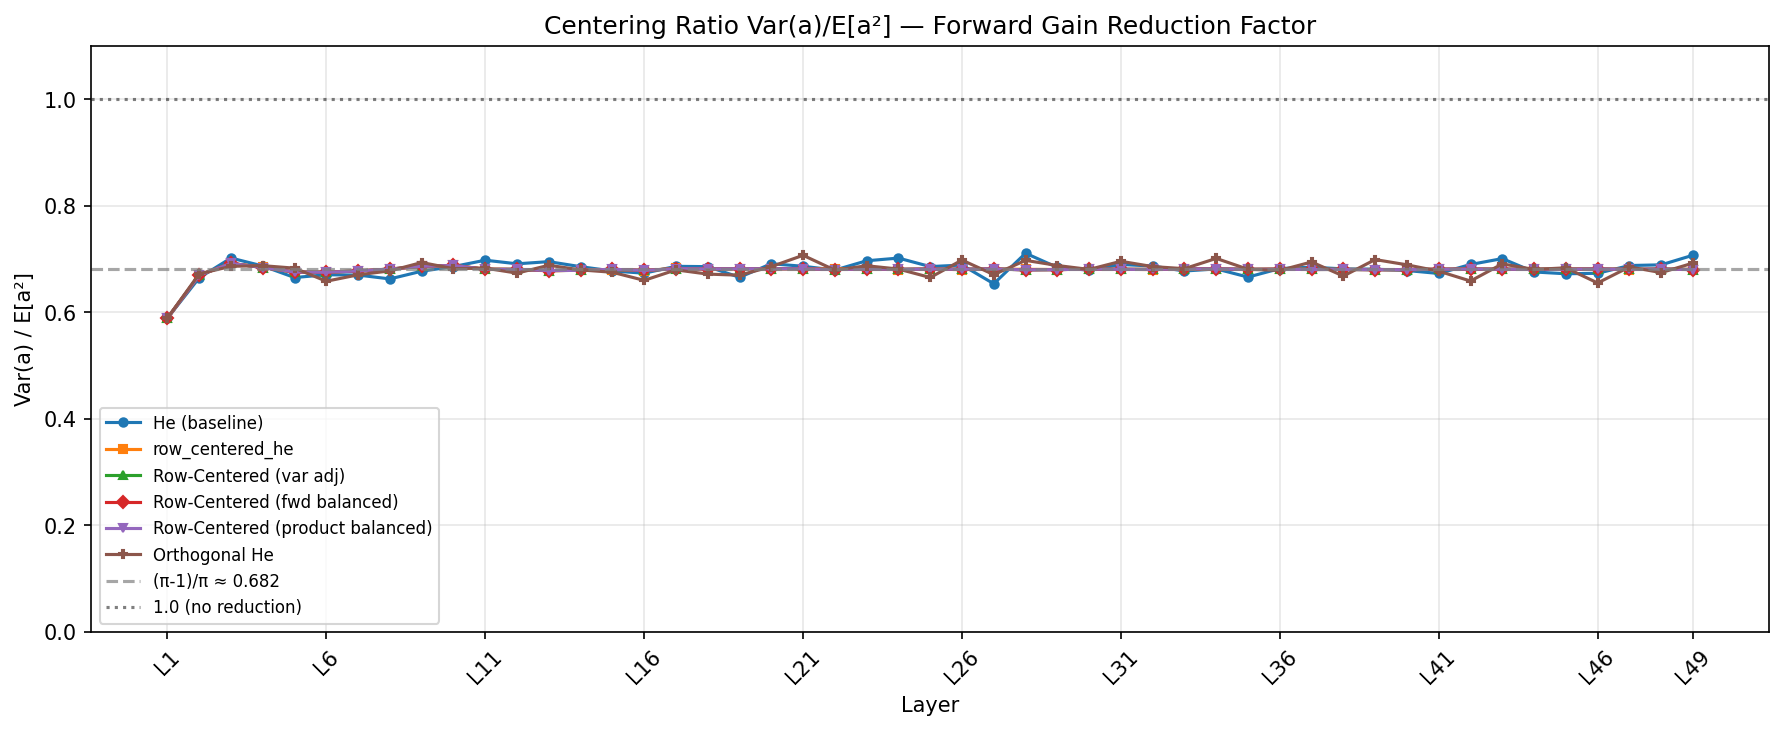
\includegraphics[width=0.85\textwidth]{figures/centering_ratio.png}
\caption{Empirical centering ratio $\Var(a)/\E[a^2]$ per layer.
  All four initializers converge to $({\pi-1})/{\pi} \approx 0.682$,
  confirming this is a universal property of post-ReLU activations.
  Source: \texttt{notebooks/06\_gradient\_diagnostics.ipynb}, Cell~10.}
\label{fig:centering_ratio}
\end{figure}

\subsection{DC/AC decomposition}
\label{sec:dc_ac}

A post-ReLU activation vector at layer~$l$ has $d$ components (one per
neuron in that layer):
$\bm{a}^{(l)} = (a_1, \dots, a_d) \in \R^d$.
Each component can be decomposed into its mean plus deviation:
\begin{equation}\label{eq:dc_ac}
  a_j = \underbrace{\bar{a}}_{\text{DC (mean)}}
      + \underbrace{(a_j - \bar{a})}_{\text{AC (deviation)}},
  \qquad \bar{a} = \frac{1}{d}\sum_{j=1}^{d} a_j.
\end{equation}

\textbf{What is ``energy''?}
In signal processing, the \emph{energy} of a signal
$\{a_1, \dots, a_d\}$ is $\sum_j a_j^2$.  The average per-element
energy is $\frac{1}{d}\sum_j a_j^2 \approx \E[a^2]$
(by the law of large numbers when $d$ is large).
This second moment measures how large the activations are on average,
regardless of sign.

\textbf{Why $\E[a^2]$ splits into DC + AC.}
From the standard variance decomposition:
\[
  \E[a^2] = \underbrace{(\E[a])^2}_{\text{DC energy}}
           + \underbrace{\Var(a)}_{\text{AC energy}}.
\]
\begin{itemize}
  \item \textbf{DC energy} $(\E[a])^2 = \sigma^2/(2\pi)$:
        This is the energy of the \emph{constant} (mean) component.
        By analogy with electrical signals, this is the ``DC'' (direct
        current) component --- a constant offset that is the
        \emph{same for all inputs}.  Whether we feed in a shoe, a shirt,
        or a bag, the mean activation $\E[a] = \sigma/\sqrt{2\pi}$
        is always the same.  It carries \textbf{zero information}
        about the class.

  \item \textbf{AC energy} $\Var(a) = \sigma^2(\pi-1)/(2\pi)$:
        This is the energy of the \emph{fluctuating} component ---
        the ``AC'' (alternating current) part that varies from input
        to input.  The deviations $(a_j - \bar{a})$ are different for
        different inputs, so they preserve the structure of the data.
        This is the \textbf{informative} part.
\end{itemize}

\noindent
The fraction of energy that is informative:
$\text{AC}/\text{total} = (\pi-1)/\pi \approx 68.2\%$.
The remaining $1/\pi \approx 31.8\%$ is uninformative DC ---
a constant offset present in every activation vector,
useless for distinguishing classes.

\subsection{Why row-centered weights are blind to DC}

\begin{proposition}[DC blindness]
\label{prop:dc_blind}
If $\sum_j W_{ij} = 0$ (row centering), then
\[
  z_i = \sum_j W_{ij}\, a_j = \sum_j W_{ij}\,(a_j - \bar{a}).
\]
The neuron's output depends only on the AC component of its input.
\end{proposition}

\begin{proof}
We split each activation into its mean plus deviation.
When row-centered weights ($\sum_j W_{ij} = 0$) multiply the mean
part, it vanishes:
\[
  \sum_j W_{ij}\, a_j
  = \sum_j W_{ij}\,\bar{a} + \sum_j W_{ij}\,(a_j - \bar{a})
  = \bar{a}\underbrace{\sum_j W_{ij}}_{=\,0}
    + \sum_j W_{ij}\,(a_j - \bar{a})
  = \sum_j W_{ij}\,(a_j - \bar{a}).
  \qedhere
\]
\end{proof}

\noindent
\textbf{Consequence for signal propagation.}
When standard He weights compute $z_i = \sum_j W_{ij}\, a_j$, the
weights see the full activation vector including its positive mean.
The variance of the pre-activation is:
\[
  \Var(z_i) = d \cdot \Var(W) \cdot \E[a^2]
  \quad\text{--- uses the \emph{full} second moment $\E[a^2]$.}
\]

When row-centered weights compute the same sum, the DC part vanishes
(Proposition~\ref{prop:dc_blind}), so effectively
$z_i = \sum_j W_{ij}(a_j - \bar{a})$.  The variance becomes:
\[
  \Var(z_i) = d \cdot \Var(W) \cdot \Var(a)
  = d \cdot \Var(W) \cdot \frac{\pi-1}{\pi}\,\E[a^2].
\]

The factor $(\pi-1)/\pi \approx 0.682$ means row-centered weights
produce pre-activations with only $68.2\%$ of the energy that He
weights produce.  This is the energy deficit that compounds across
layers.

% ──────────────────────────────────────────────────────────────────
\section{Forward Gain Derivation}
\label{sec:fwd_gain_derivation}

\subsection{Standard He: forward gain $= 1$}

For a He-initialized layer (no centering), the expected output energy
is:
\begin{equation}\label{eq:he_energy}
  \E[(a^{(l)})^2]
  = \underbrace{\Var(W) \cdot d}_{= (2/d)\cdot d = 2}
  \cdot \underbrace{\frac{1}{2}}_{\text{ReLU survival}}
  \cdot \E[(a^{(l-1)})^2]
  = \E[(a^{(l-1)})^2].
\end{equation}
The forward gain is $g_{\mathrm{fwd}}^{\mathrm{He}} = \sqrt{\E[(a^{(l)})^2] / \E[(a^{(l-1)})^2]} = 1$.

\subsection{Row-centered: forward gain $= \sqrt{(\pi-1)/\pi}$}

The key step: in the He derivation~\eqref{eq:he_energy}, the factor
$\E[(a^{(l-1)})^2]$ appears because He weights see the \emph{full}
activation energy.  For row-centered weights, we must replace this
with $\Var(a^{(l-1)})$ (because of DC blindness,
Proposition~\ref{prop:dc_blind}).  Since
$\Var(a) = \frac{\pi-1}{\pi}\,\E[a^2]$
(Proposition~\ref{prop:centering_ratio}), we get the extra factor
$(\pi-1)/\pi$.

For a row-centered layer with variance-adjusted weights
($\Var(W_{ij}) = 2/d$):

\begin{equation}\label{eq:rc_energy}
  \E[(a^{(l)})^2]
  = \underbrace{\Var(W) \cdot d \cdot \frac{1}{2}}_{= 1}
  \cdot \underbrace{\Var(a^{(l-1)})}_{\text{only AC visible}}
  = \Var(a^{(l-1)})
  = \frac{\pi-1}{\pi}\,\E[(a^{(l-1)})^2].
\end{equation}

This gives a multiplicative recurrence in the energy:
\[
  \E[(a^{(l)})^2] = \frac{\pi-1}{\pi}\,\E[(a^{(l-1)})^2].
\]
At every layer, row-centered weights produce activations whose energy
is $(\pi-1)/\pi \approx 0.682$ times the energy of the previous
layer's activations.  The signal shrinks at every layer.

The forward gain is the ratio of \textbf{amplitudes} (RMS), not energies:
\begin{equation}\label{eq:rc_fwd_gain}
  \boxed{
  g_{\mathrm{fwd}}^{\mathrm{RC}}
  = \sqrt{\frac{\E[(a^{(l)})^2]}{\E[(a^{(l-1)})^2]}}
  = \sqrt{\frac{\pi-1}{\pi}}
  \approx 0.826.
  }
\end{equation}

\begin{remark}[Amplitude vs.\ energy ratio]
\label{rem:amplitude}
The forward gain is defined as
$g_{\mathrm{fwd}} = \rms(A^{(l)}) / \rms(A^{(l-1)})$,
which is a ratio of \emph{amplitudes} (RMS values).
Since $\rms^2 \propto \E[a^2]$ (energy), we have
\[
  g_{\mathrm{fwd}}^2
  = \frac{\E[(a^{(l)})^2]}{\E[(a^{(l-1)})^2]}
  = \frac{\pi-1}{\pi}
  \approx 0.682.
\]
Taking the square root:
$g_{\mathrm{fwd}} = \sqrt{0.682} \approx 0.826$.

\emph{Analogy:} if you halve the power of a light bulb
(energy ratio~$= 1/2$), the brightness (amplitude) drops by
$\sqrt{1/2} \approx 0.707$, not by~$1/2$.
Similarly, an energy ratio of $0.682$ corresponds to an amplitude
ratio of $\sqrt{0.682} = 0.826$.
\end{remark}

\begin{figure}[h]
\centering
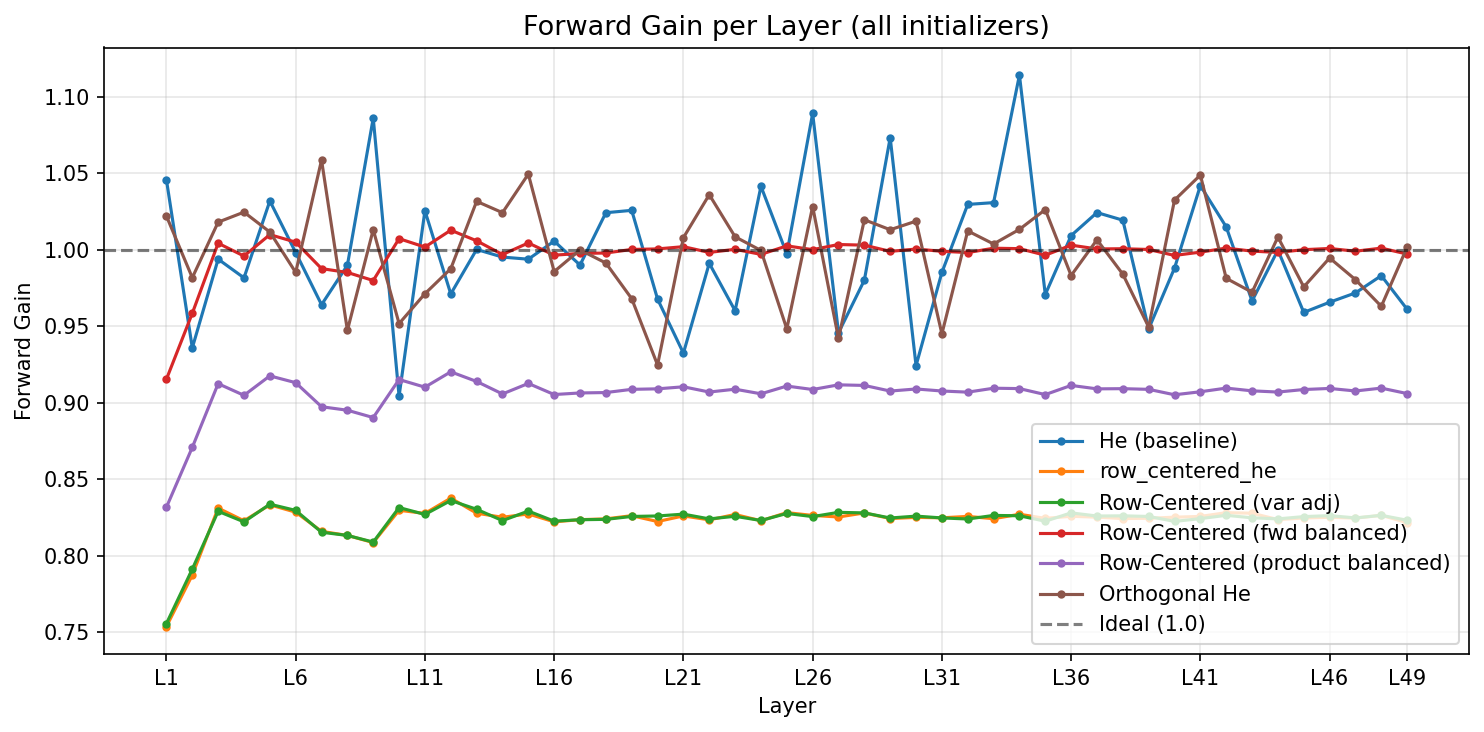
\includegraphics[width=0.85\textwidth]{figures/forward_gain_per_layer.png}
\caption{Forward gain per layer for four initializers (50 hidden layers,
  width~784, Fashion-MNIST).  He and RC~fwd-balanced achieve gain $\approx 1.0$;
  RC~var-adj and \texttt{row\_centered\_he} are locked at $\approx 0.826$.
  Source: \texttt{notebooks/06\_gradient\_diagnostics.ipynb}, Cell~8.}
\label{fig:forward_gain}
\end{figure}

\begin{figure}[h]
\centering
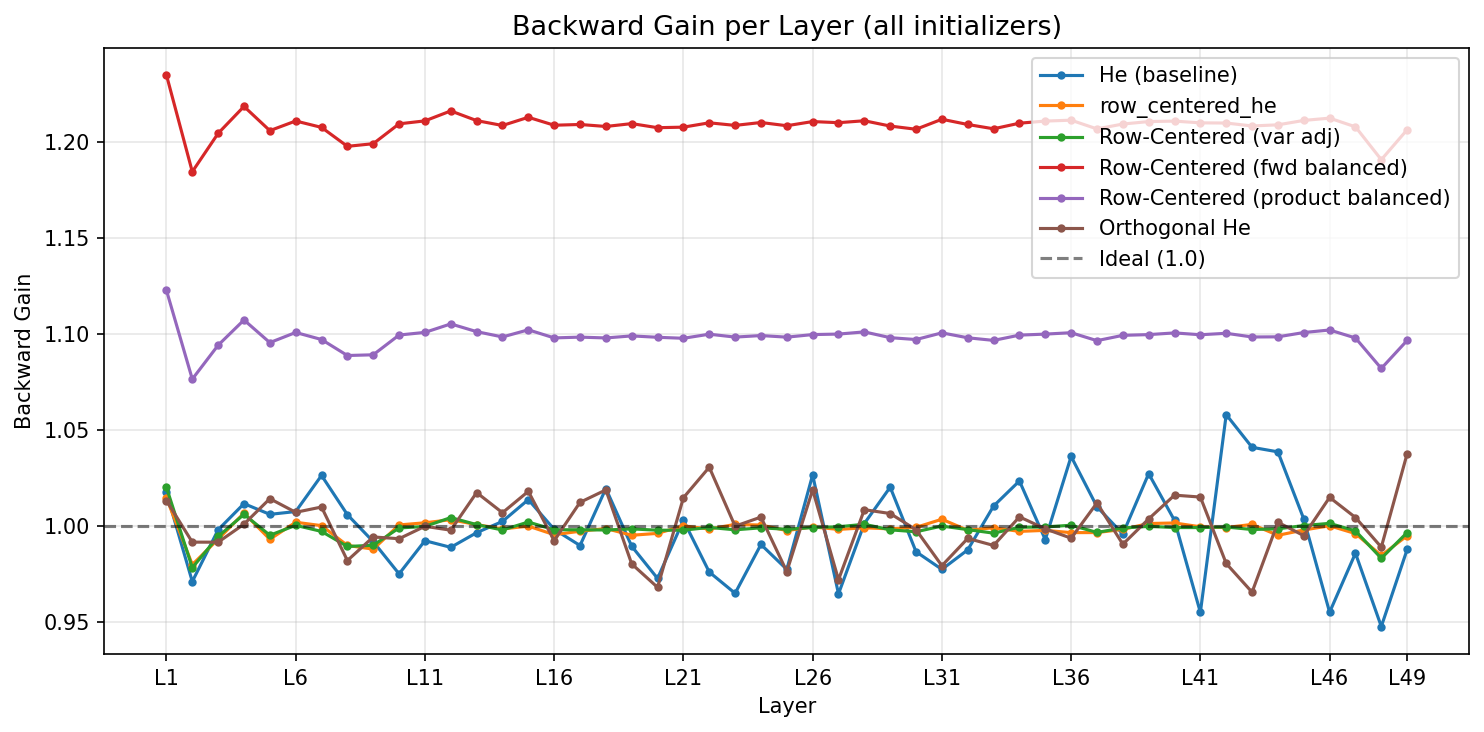
\includegraphics[width=0.85\textwidth]{figures/backward_gain_per_layer.png}
\caption{Backward gain per layer.  He, RC~var-adj, and
  \texttt{row\_centered\_he} all have gain $\approx 1.0$.
  RC~fwd-balanced has gain $\approx 1.21$ --- error signals
  explode at $1.21^{50} \approx 1.3 \times 10^4$.
  Source: \texttt{notebooks/06\_gradient\_diagnostics.ipynb}, Cell~8.}
\label{fig:backward_gain}
\end{figure}

\subsection{Compounding over depth}

Over $L$ layers:
\begin{equation}\label{eq:compounding}
  \rms(a^{(L)}) = \left(\frac{\pi-1}{\pi}\right)^{L/2} \rms(a^{(0)})
  \approx 0.826^L \cdot \rms(a^{(0)}).
\end{equation}

\begin{center}
\begin{tabular}{cc}
\toprule
Depth $L$ & Forward attenuation $0.826^L$ \\
\midrule
10 & $0.147$ \quad ($6.8\times$ decay) \\
20 & $0.022$ \quad ($46\times$ decay) \\
50 & $7.1 \times 10^{-5}$ \quad ($14{,}000\times$ decay) \\
\bottomrule
\end{tabular}
\end{center}

By layer~50, the activations are $14{,}000$ times smaller than the
input.  From~\eqref{eq:grad_magnitude}, the gradient at layer~$l$ is
proportional to $\|\bm{a}^{(l-1)}\|$, so later layers receive
vanishingly small gradients.

% ──────────────────────────────────────────────────────────────────
\section{Why the Backward Gain Is Unaffected}
\label{sec:bwd_gain}

The backward pass propagates the error signal via:
\begin{equation}\label{eq:backward}
  \bm{\delta}^{(l)}
  = \bigl(W^{(l+1)}\bigr)^\top \bm{\delta}^{(l+1)}
    \odot \sigma'(\bm{z}^{(l)}),
\end{equation}
where $\sigma'(\bm{z}^{(l)}) = \mathbf{1}[\bm{z}^{(l)} > 0]$ is the
ReLU derivative (binary mask).

If $W$ is row-centered ($\sum_j W_{ij} = 0$), then $W^\top$ is
\emph{column-centered} ($\sum_i W_{ij} = 0$ for each column~$j$).
Applying $W^\top$ to $\bm{\delta}^{(l+1)}$ gives:
\[
  (W^\top \bm{\delta})_j = \sum_i W_{ij}\,\delta_i.
\]
The centering of columns means this is blind to the mean of
$\bm{\delta}^{(l+1)}$.  However, unlike post-ReLU activations, the
error signal $\bm{\delta}$ has \textbf{near-zero mean} (it contains
both positive and negative values).  Therefore:
\[
  \frac{\Var(\delta)}{\E[\delta^2]}
  = 1 - \frac{(\E[\delta])^2}{\E[\delta^2]}
  \approx 1,
\]
and the column centering of $W^\top$ has negligible effect on the
backward signal energy.

\begin{proposition}[Forward-backward gain ratio]
\label{prop:fb_ratio}
For row-centered initialization with any weight variance:
\begin{equation}\label{eq:fb_ratio}
  \frac{g_{\mathrm{fwd}}}{g_{\mathrm{bwd}}}
  = \sqrt{\frac{\pi-1}{\pi}}
  \approx 0.827.
\end{equation}
This ratio is \textbf{independent of the weight variance}.
\end{proposition}

This is the fundamental coupling: the forward and backward gains
are locked in a fixed ratio.  No scalar variance adjustment can make
both equal to~1 simultaneously.

% ──────────────────────────────────────────────────────────────────
\section{Empirical Confirmation: Variance Sweep}
\label{sec:var_sweep}

We sweep the variance factor for row-centered initialization from
$1.5/d$ to $3.0/d$:

\begin{center}
\begin{tabular}{cccc}
\toprule
Variance factor & Median fwd gain & Median bwd gain & Ratio F/B \\
\midrule
$1.5/d$ & 0.715 & 0.865 & \textbf{0.827} \\
$2.0/d$ (He) & 0.826 & 0.999 & \textbf{0.827} \\
$2.5/d$ & 0.923 & 1.116 & \textbf{0.827} \\
$3.0/d$ & 1.011 & 1.223 & \textbf{0.827} \\
\bottomrule
\end{tabular}
\end{center}

The ratio $g_{\mathrm{fwd}}/g_{\mathrm{bwd}} = 0.827$ is constant
across all variance factors, confirming
Proposition~\ref{prop:fb_ratio}.

\textbf{Interpretation:}
\begin{itemize}
  \item At $\Var = 2.0/d$: backward gain $= 1.0$ (healthy), but
        forward gain $= 0.826$ (activations vanish).
  \item At $\Var \approx 2.93/d$: forward gain $= 1.0$ (healthy), but
        backward gain $= 1.21$ (error signals explode:
        $1.21^{50} \approx 1.3 \times 10^4$).
  \item No variance gives both $= 1$.
\end{itemize}

\section{The Coupling Formula}
\label{sec:fwd_bwd_coupling}

Writing the forward gain as $g_{\mathrm{fwd}} = r \cdot s$ where
$r = \sqrt{(\pi-1)/\pi} \approx 0.826$ is the structural centering
factor and $s$ depends on the weight variance, and the backward gain as
$g_{\mathrm{bwd}} = s$:

\begin{equation}\label{eq:coupling}
  \frac{g_{\mathrm{fwd}}}{g_{\mathrm{bwd}}} = r \approx 0.826
  \quad\text{always.}
\end{equation}

\begin{itemize}
  \item $s = 1$ (He variance, \texttt{var\_adj}):
        $g_{\mathrm{fwd}} = 0.826$, $g_{\mathrm{bwd}} = 1.0$
        $\Rightarrow$ activations vanish.
  \item $s = 1/r \approx 1.21$ (\texttt{fwd\_balanced}):
        $g_{\mathrm{fwd}} = 1.0$, $g_{\mathrm{bwd}} = 1.21$
        $\Rightarrow$ error signals explode.
  \item Any $s$ in between: both are off from~1.
\end{itemize}

\textbf{This is why geometry (requiring row centering) and gradient
stability (requiring gain $\approx 1$) conflict.}

% ──────────────────────────────────────────────────────────────────
\section{Single vs.\ Multi-Sample: The Trap Is Structural}
\label{sec:single_multi}

To verify that the gradient non-uniformity is not a statistical
artifact of batch aggregation, we compare gradient profiles using
$n = 1$ vs.\ $n = 2000$ samples.

\begin{center}
\begin{tabular}{lcc}
\toprule
Initializer & Log-scale correlation & Interpretation \\
\midrule
He & 0.86 & Noisier (no centering stabilization) \\
RC var-adj & 0.98 & Same pattern \\
RC fwd-balanced & 0.98 & Same pattern \\
\bottomrule
\end{tabular}
\end{center}

The row-centered variants show correlation $> 0.97$ between single-sample
and batch gradient profiles.  The gradient decay pattern is identical
whether we use one data point or two thousand.

\textbf{Conclusion:} The gradient non-uniformity is \textbf{structural}
--- it comes from the weight matrices and the ReLU activation, not from
data aggregation.

% ──────────────────────────────────────────────────────────────────
\section{ReLU Survival Is Not the Issue}
\label{sec:relu_survival}

All three initializers show ReLU survival rates of approximately
$50\% \pm 2\%$ across all layers:

\begin{itemize}
  \item He: $50\% \pm 1.7\%$ (higher noise)
  \item RC var-adj: $50\% \pm 0.4\%$ (tighter due to centering)
  \item RC fwd-balanced: $50\% \pm 0.4\%$
\end{itemize}

Row centering does \textbf{not} kill more neurons than standard He.
The gradient trap is not about dead neurons --- it is about the
\emph{positive mean} of surviving activations (the DC component that
row-centered weights cannot see).
